\documentclass[12pt, letterpaper, twoside, titlepage]{article}
% font size could be 10pt (default), 11pt or 12 pt
% paper size coulde be letterpaper (default), legalpaper, executivepaper,
% a4paper, a5paper or b5paper
% side coulde be oneside (default) or twoside 
% columns coulde be onecolumn (default) or twocolumn
% graphics coulde be final (default) or draft 
%
% titlepage coulde be notitlepage (default) or titlepage which 
% makes an extra page for title 
% 
% paper alignment coulde be portrait (default) or landscape 
%
% equations coulde be 
%   default number of the equation on the rigth and equation centered 
%   leqno number on the left and equation centered 
%   fleqn number on the rigth and  equation on the left side
%

\usepackage{graphicx}
\usepackage{hyperref}
\usepackage[left=3cm, right=3cm, top=3cm]{geometry}
\usepackage{listings}
\usepackage{color}
\definecolor{codegreen}{rgb}{0,0.6,0}
\definecolor{codegray}{rgb}{0.5,0.5,0.5}
\definecolor{codepurple}{rgb}{0.58,0,0.82}
\definecolor{backcolour}{rgb}{0.95,0.95,0.92}

\lstdefinestyle{mystyle}{                                                                                                        
    backgroundcolor=\color{backcolour},                                                                                                     
    commentstyle=\color{codegreen},                                                                           
    keywordstyle=\color{magenta},                                                                                 
    numberstyle=\tiny\color{codegray},                                                                                             
    stringstyle=\color{codepurple},                                                                                     
    basicstyle=\footnotesize,                                                                                              
    breakatwhitespace=false,
    breaklines=true,
    captionpos=b,
    keepspaces=true,
    numbers=left,
    numbersep=5pt,
    showspaces=false,
    showstringspaces=false,
    showtabs=false,
    tabsize=2
}

\lstset{style=mystyle} 

\usepackage{mathpazo,amsmath}
\def\inch#1{#1''}
\usepackage{fancyhdr}
 
\pagestyle{fancy}
\fancyhf{}
\rhead{JLAB Beam Accounting Tools}
\lhead{\today}
\cfoot{\thepage}
	
\title{\textit{ Beam accounting in Hall-C}}
\author{Lorenzo Zana  \\
	Jefferson Lab  \\
	\and 
	Rad. Control Department \\
	Jefferson Lab \\
	}

\date{\today} 
% \date{\today} date coulde be today 
% \date{25.12.00} or be a certain date
% \date{ } or there is no date 
\begin{document}
% Hint: \title{what ever}, \author{who care} and \date{when ever} could stand 
% before or after the \begin{document} command 
% BUT the \maketitle command MUST come AFTER the \begin{document} command! 
\maketitle


%\tableofcontents % create a table of contens 



\section{Introduction}
Radiation budget need to be evaluated with every experiment. In this study it is shown the results for run group E12-09-011,E12-09-017,E12-09-002 that will run in Hall-C during the Fall of 2018. In order to evaluate this, I have developed different tools that will permit to speed up similar analysis for Hall-C and other Halls. The scope of this technical note is to show the status of this tools and the results obtained analyzing the results from simulations for this experiment.\\
During an experiment in Hall-C, in order to account for beam exposure and activation in the Hall, with normal configuration, one will need to take into account the radiation in the enclosure of the beam-line. Multiple targets will run multiple times with different intensities. Radiation budget for this experiment will be a cumulative answer from all these configurations. Fluka has the key feature to easily obtain statistics for these low process without too high computing power and can calculate activation dose at different times from beam exposure.
\section{Getting info from the CAD design}
Different experiments will have a different beam-line setup.  Since too much detail will be difficult to debug and will also consistently slow-down the simulation, it is important to transfer just the important part of the setup for radiation simulation in FLUKA. In order to achieve this, simplified information regarding the beam enclosure where filtered from the design and transformed in information useful for the FLUKA model. Different materials for the flange in the beam-line (bolts, nuts, washers) had their weight determined and a local material was created for each flange in order to address local activation. The other relevant information was then transferred to a text file with:
\begin{itemize} 
\item Start Z (cm)
\item Stop Z (cm)
\item Outer Radius (cm)
\item Thickness (cm)
\item Inner Radius (cm)
\item Weight (lbs)
\item Length (cm)
\item Material
\end{itemize}
See table \ref{tab:1} for the info used in this example.
\begin{center}
\begin{table}[!ht]
\begin{scriptsize}
\begin{tabular}{ | l | l | l | l | l | l | l | l | }
  \hline\noalign{\smallskip}
  Start Z(cm) &	Stop Z(cm) &	Outer R(cm) &	Thickness(cm) &	Inner R(cm) &	Weight(lbs) &	Length(cm) &	Material \\
\hline
  69.85 & 71.12 &	3.50012	&	1.651 &  1.84912 &		0.48768	&  1.27	& 6061-T6Alum \\
  71.12 & 78.8924 & 2.14884 & 0.29972 & 		1.84912 &   0.4953 & 7.7724 & 6061-T6Alum \\
78.8924 & 	258.5212 & 2.54 & 		0.47752 &   2.06248 & 9.53008 & 179.6288 & 6061-T6Alum \\
258.5212 & 260.096 & 	3.65252 & 		1.5875 &   2.06502 & 0.65278 & 1.5748 & 	6061-T6Alum \\
260.096 & 	417.449 & 	3.65252 & 		0.51816 &   3.13436 & 25.146 & 157.353 & 	6061-T6Alum \\
417.449 & 	419.1762 & 7.06628 & 		3.92938 &   3.1369 & 3.11404 & 1.7272 & 	6061-T6Alum \\
419.1762 & 422.6687 & 6.35 & 		1.5875 &   4.7625 & 4.01066 & 3.4925 & 	6061-T6Alum \\
422.6687 & 804.6212 & 6.35 & 		0.635 &   5.715 & 	139.573 & 381.9525 & 6061-T6Alum \\
804.6212 & 806.8437 & 9.017 & 		2.54 &   6.477 & 	4.064 & 2.2225 & 	6061-T6Alum \\
806.8437 & 868.68 & 	8.89 & 		0.635 &   8.255 & 	32.8422 & 61.8363	 & 6061-T6Alum \\
868.68 & 	870.966 & 	13.6525 & 		5.3975 &   8.255 & 	11.3284 & 2.286 & 	6061-T6Alum \\
870.9787 & 873.5187 & 13.6525 & 		3.7084 &   9.9441 & 29.1338 & 2.54 & 	347SS \\
873.5187 & 886.4219 & 10.16 & 		0.2159 &   9.9441 & 7.747 & 12.9032 & 	347SS \\
886.4219 & 888.9619 & 13.6525 & 		3.7084 &   9.9441 & 29.1338 & 2.54 & 	347SS \\
888.9619 & 891.8194 & 13.6525 & 		2.8575 &   10.795 & 8.88238 & 2.8575 & 	6061-T6Alum \\
891.8194 & 1087.3994 & 13.6525 & 		0.9525 &   12.7 & 	229.7811 & 	195.58 & 6061-T6Alum \\
1087.3994 & 1090.2569 & 22.86 & 		10.16 &   12.7 & 	43.59656 & 	2.8575 & 6061-T6Alum \\
1090.2569 & 1094.0669 & 29.845 & 		14.605 &   15.24 & 	112.93348 & 	3.81 & 6061-T6Alum \\
1110.5261 & 1114.3361 & 29.845 & 		14.68374 &  15.16126 & 114.3 & 		3.81 & 6061-T6Alum \\
1114.3361 & 1265.4915 & 16.1925 & 		1.03124 &   15.16126 & 232.16108 & 	151.1554 & 6061-T6Alum \\
1265.4915 & 1268.349 & 22.86 & 		7.69874 &   15.16126 & 38.49878 & 	2.8575 & 	6061-T6Alum \\
1268.349 & 1273.175 & 22.86 & 		6.985 &   15.875 & 59.90844 & 	4.826 & 	6061-T6Alum \\
1273.175 & 1648.46 & 	22.86 & 		0.9525 &   21.9075 & 756.6279 & 	375.285 & 	6061-T6Alum \\
1648.46 & 	1653.2225 & 30.48 & 		8.5725 &   21.9075 & 97.58934 & 	4.7625 & 	6061-T6Alum \\
1653.2225 & 1657.985 & 30.48 & 		7.62 &   22.86 & 	89.78138 & 	4.7625 & 	6061-T6Alum \\
1657.985 & 1896.7958 & 30.48 & 		0.9525 &   29.5275 & 646.03376 & 	238.8108 & 6061-T6Alum \\
1896.7958 & 1901.5583 & 40.64 & 		11.1125 &   29.5275 & 162.39744 & 	4.7625 & 	6061-T6Alum \\
1901.5583 & 1906.3208 & 40.64 & 		11.1125 &   29.5275 & 162.39744 & 	4.7625 & 	6061-T6Alum \\
1906.3208 & 2145.3983 & 30.48 & 		0.9525 &   29.5275 & 646.75512 & 	239.0775 & 6061-T6Alum \\
2145.3983 & 2150.1608 & 40.64 & 		11.1125 &   29.5275 & 162.39744 & 	4.7625 & 	6061-T6Alum \\
2150.1608 & 2156.2441 & 40.64 & 		11.1125 &   29.5275 & 207.49006 & 	6.0833 & 	6061-T6Alum \\
2156.2441 & 2534.2977 & 30.48 & 		0.9525 &   29.5275 & 1026.45718 & 	378.0536 & 6061-T6Alum \\
2534.2977 & 2539.0602 & 40.64 & 		11.1125 &   29.5275 & 162.39744 & 	4.7625 & 	6061-T6Alum \\
2539.0602 & 2543.8227 & 40.64 & 		11.1125 &   29.5275 & 162.39744 & 	4.7625 & 	6061-T6Alum \\
2543.8227 & 2608.4911 & 30.48 & 		0.9525 &   29.5275 & 175.58258 & 	64.6684 & 	6061-T6Alum \\
2608.4911 & 2613.2536 & 40.64 & 		11.1125 &   29.5275 & 162.39744 & 	4.7625 & 	6061-T6Alum \\
2613.2536 & 2619.95158 & 40.64 & 		11.1125 &   29.5275 & 474.4466 & 	6.69798 & 	304SS \\
2619.95158 & 2667.12192 & 29.845 & 		0.3175 &   29.5275 & 493.8268 & 	47.17034 & 304SS \\
2667.12192 & 2671.88442 & 40.64 & 		11.1125 &   29.5275 & 474.4466 &  4.7625 & 	304SS \\

  \noalign{\smallskip}\hline
\end{tabular}
\end{scriptsize}
\caption{Beam-line properties to be transferred in Fluka}
\label{tab:1}
\end{table}
\end{center}
A bash script \cite{code} will help create the full geometry of the beam-line, with each region divided by each different materials, all with the correct spacing needed by Fluka. This will help to speed up the implementation of a new beam pipe design into the Hall.





\section{Running the simulation in the farm system at Jlab}
The different target cells where created in different input files: These will be used for creating the multiple different outputs. The info for the run period were screened and put in a input file containing:
\begin{itemize}
\item Target
\item hours
\item current($\mu$A)
\item Energy(GeV)
\end{itemize}
See Table \ref{tab:2} for the beam time for this experiment.

\begin{table}[!ht]
\begin{center}
\begin{tabular}{ | l | c | r | c | c | }
  \hline\noalign{\smallskip}

n &	Target	&	hours	&	current($\mu$A) &	Energy(GeV) \\
\hline
1 & $H_2$ & 	108.0 & 	70 & 	9.4 \\
2 & Al	 & 12.0 & 	40 & 	9.4 \\
3 & $H_2$ & 	31.2 & 	70 & 	6.4 \\
4 & Al & 	4.8 & 	40 & 	6.4 \\
5 & $H_2$	 & 74.4 & 	35 & 	4.9 \\
6 & Al & 	9.6 & 	40 & 	4.9 \\
7 & $H_2$ & 	108.0 & 	35 & 	3.8 \\
8 & Al & 	12.0 & 	40 & 	3.8 \\
9 & $H_2$ & 	240.0 & 	70 & 	10.6 \\
10 & Al & 	26.4 & 	40 & 	10.6 \\
11 & $H_2$ & 	240.0 & 	70 & 	8.5 \\
12 & Al & 	26.4 & 	40 & 	8.5 \\
13 & $H_2$ & 	57.6 & 	50 & 	10.6 \\
14 & $H_2$ & 	45.6 & 	10 & 	10.6 \\
15 & $D_2$ & 	134.4 & 	50 & 	10.6 \\
16 & $D_2$ & 	91.2 & 	25 & 	10.6 \\
17 & $D_2$ & 	45.6 & 	10 & 	10.6 \\
18 & Al & 	36.0 & 	40 & 	10.6 \\
19 & $H_2$ & 	12.0 & 	50 & 	8.5 \\
20 & $D_2$ & 	12.0 & 	50 & 	8.5 \\
21 & Al & 	2.4 & 	40 & 	8.5 \\

  \noalign{\smallskip}\hline
\end{tabular}
\caption{Prospected beam time for the full experiment}
\label{tab:2}
\end{center}
\end{table}


These info will be convoluted in the different input files in order to create the different configurations needed. In order to obtain the desired statistic and well use the structure of the Jlab farm computing system, each configuration will run multiple times. In order to speed up this procedure of creating multiple inputs, each configuration file will have similar structure, with the info that need to be modified at the same line. What the submission script \cite{code} does is:
\begin{itemize}
\item The current is given in $\mu$A and will need to be transferred in number of particle per seconds for the activation with this configuration
\item The energy will be replaced with the correct one for each configuration
\item The hours of running with each configuration will be transformed in seconds and divided in 5 parts. In order to assume a more accurate accelerator efficiency during run time, each of the 5 time ranges of beam exposure will be followed by the same time range of no beam. This will give a 55\% efficiency.
\item The integrated beam exposure  will be recorded for each time in order to have a final number to be used in the normalization later (Fluka calculates some of their obervable in (quantity measured)/(incident beam particle) ).
\item The full activation of the  experiment is a convolution of the different configurations reacirded at the sane time after all the different targets were exposed. The time of activation from beam exposure at the end of the experiment will depend of the time that is left in the experiment: For this reason, in order to get the correct time at each configuration, one start the time accounting from the last target exposed, and build the correct time delay for each configuration adding each contribution to the full exposure.
\item The activation was then calculated at different time from beam exposure (1 hour, 12 hours, 1 day, 1 week, 1 month) for each target exposure and for the full experiment exposure, using different times for each targets, decided from the algorithm explained in the previous point
\item For each configuration multiple simulation were created. The random seed was created and modified for each simulation in order to assure that each simulation was statistically independent.
\end{itemize}

\section{Analyzing the results}
In order to analyze the results, we will need to take into account how these results are recorded in Fluka. The activation is recorded in pSv/second, rather than the dose and the 1 MeV neutron equivalent flux on Silicon it is recorded per incident beam particle.
\subsection{Activation studies}
For activation studies we will need to keep in mind that the results are recorded for each target in dose equivalent pSv/second. In order to get the activation for all the targets at the times of observation after the end of the all experiment, One will need to add all the different contribution from the the different running times with the different targets, where the observation time window has been shifted correctly. While averaging the different activation from different targets, it is important to keep the same number of simulations with each configuration. Scaling the results with the total number of configuration run will then give the final result. 


\subsection{Accumulated dose and 1 MeV neutron equivalent flux}
For these observable the recorded data for each target is done for single incident particle. In order to get the right sample of simulations for the experiment one will need to scale each configuration with the number of incident particle that was run for each configuration. Since the data is cumulative, a full average over this weighted sample will give the dose per electron for the full experiment. 


\section{Results}
Results were calculated after each target and after the full experiment. Activation was calculated in the volume surrounding the beam line with a granularity of a cube of 10cm size:
\begin{itemize}
\item Z: from -2m from the target to the beam dump at the end of the wall
\item X: from -2m from the target to 2m
\item Y from the floor($- \sim 4m$) to 1m over the target.
\end{itemize}
The accumulated radiation level is projected on a plane at 1.5m from the ground and observed in planes perpendicular to the beam-line at different distance from the target: 1.1m, 3.0m, 5.0m, 10.0m, 15.0m, 20.0m. Radiation levels are also projected on the beam-pipe and the walls. The radiation is averaged over a cube of 10cm in size. In Figure \ref{fig:dose_acc} it is shown the expected accumulated dose after the full experiment. In order to address electronics radiation damage, one can consider also the 1 MeV equivalent neutron flux on Silicon per $cm^2$: This is shown in Figure \ref{fig:1mev_acc}. From Figure \ref{fig:act1h} to Figure \ref{fig:act1m} it is shown the expected activation in the Hall after the experiment is finished. The activation is estimated after  1 hour, 12 hours, 1 day, 1 week, 1 month from beam exposure and is expressed in mrem/hour. 
\begin{figure}[!ht]
  \begin{center}
    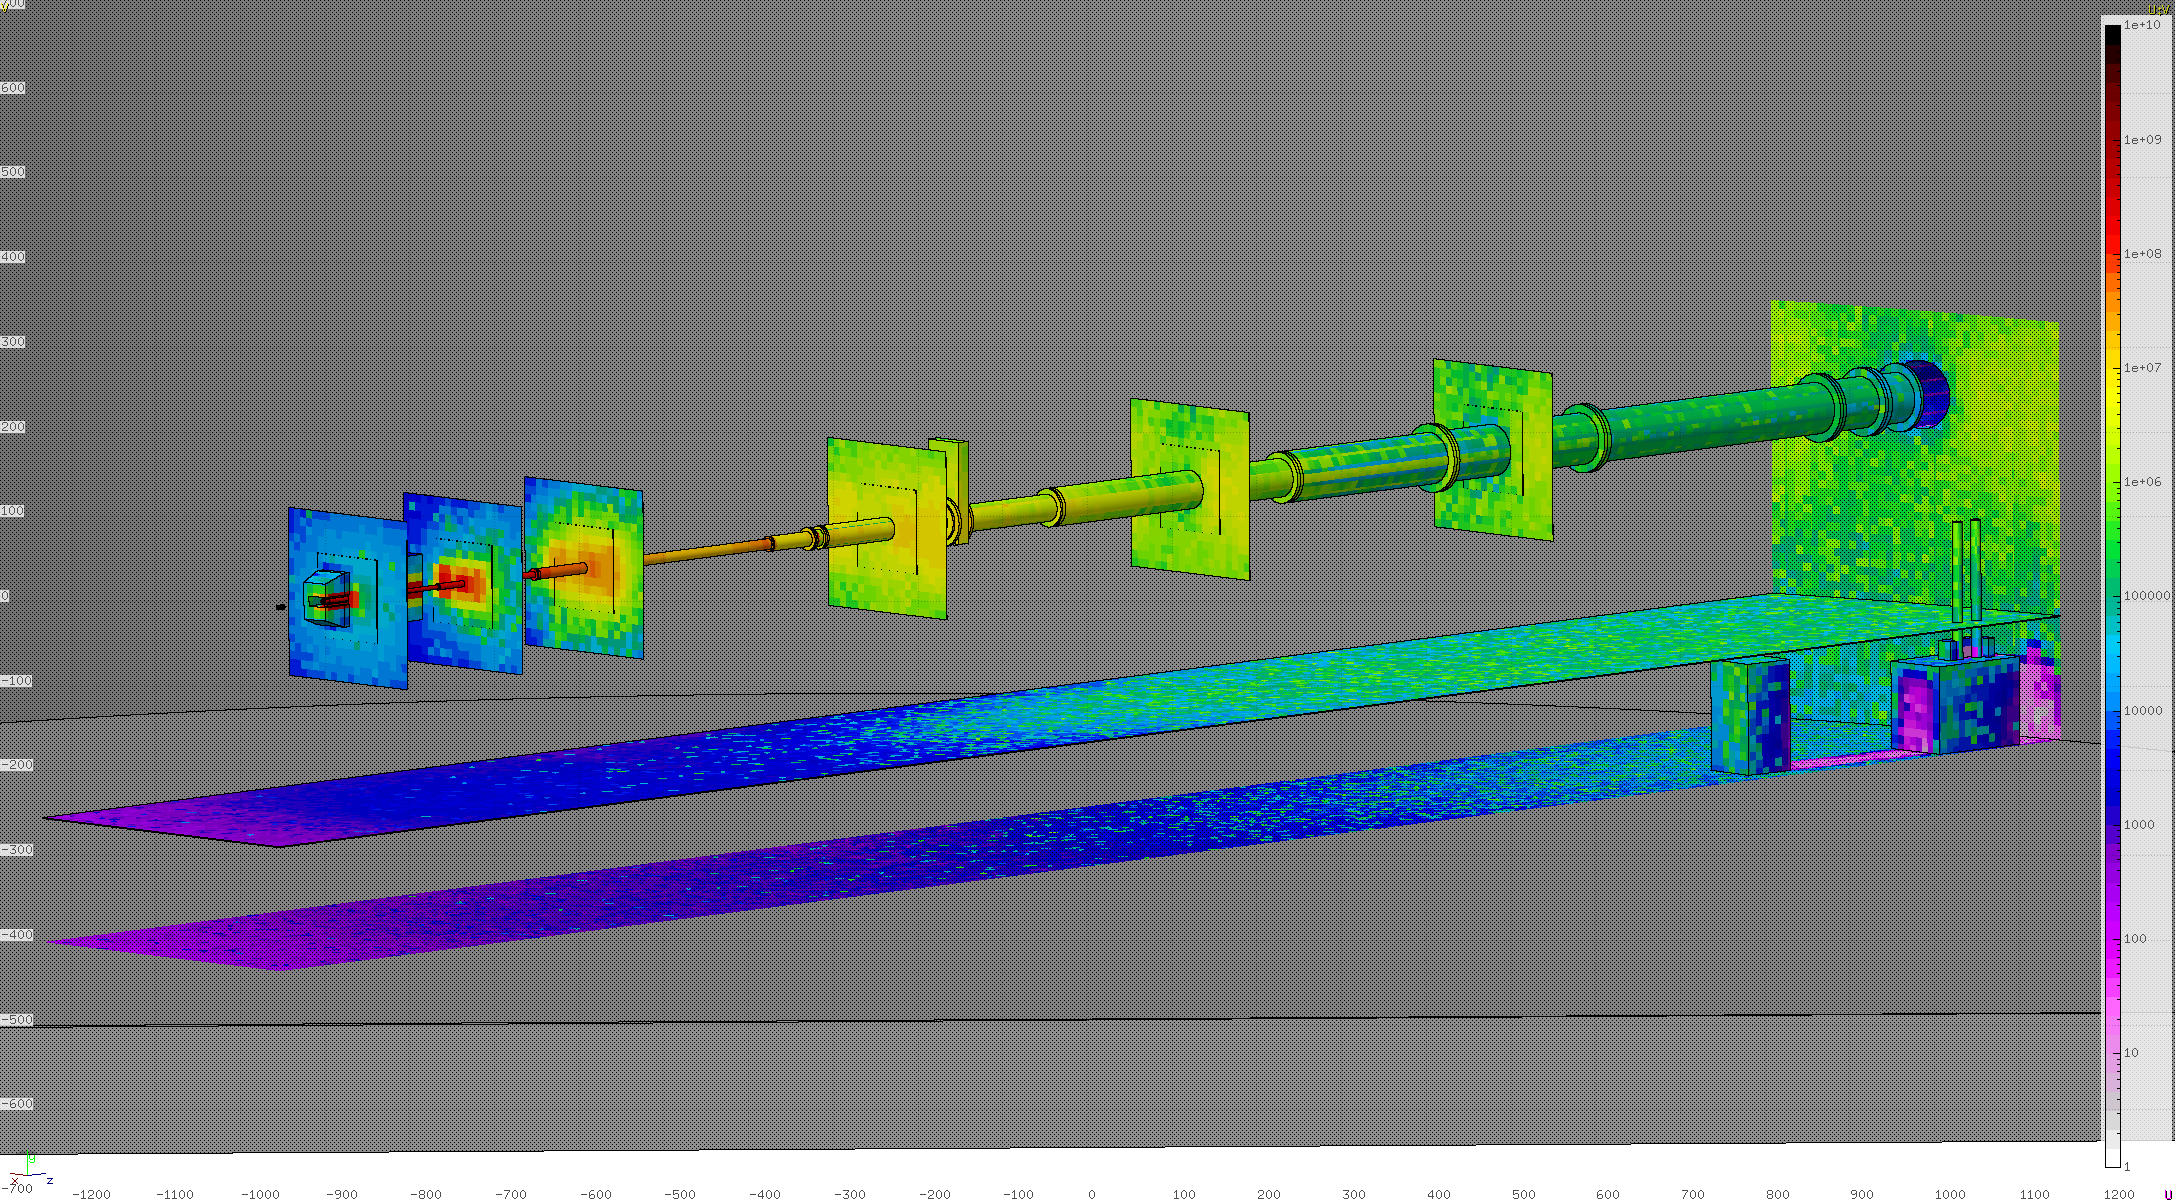
\includegraphics[width=\textwidth]{Pictures/accumulated_dose_rad.png} \\
    \caption{Accumulated Dose (rad) cumulative for the full exposure as shown in Table\ref{tab:2}.   }
    \label{fig:dose_acc}
  \end{center}
\end{figure}


\begin{figure}[!ht]
  \begin{center}
    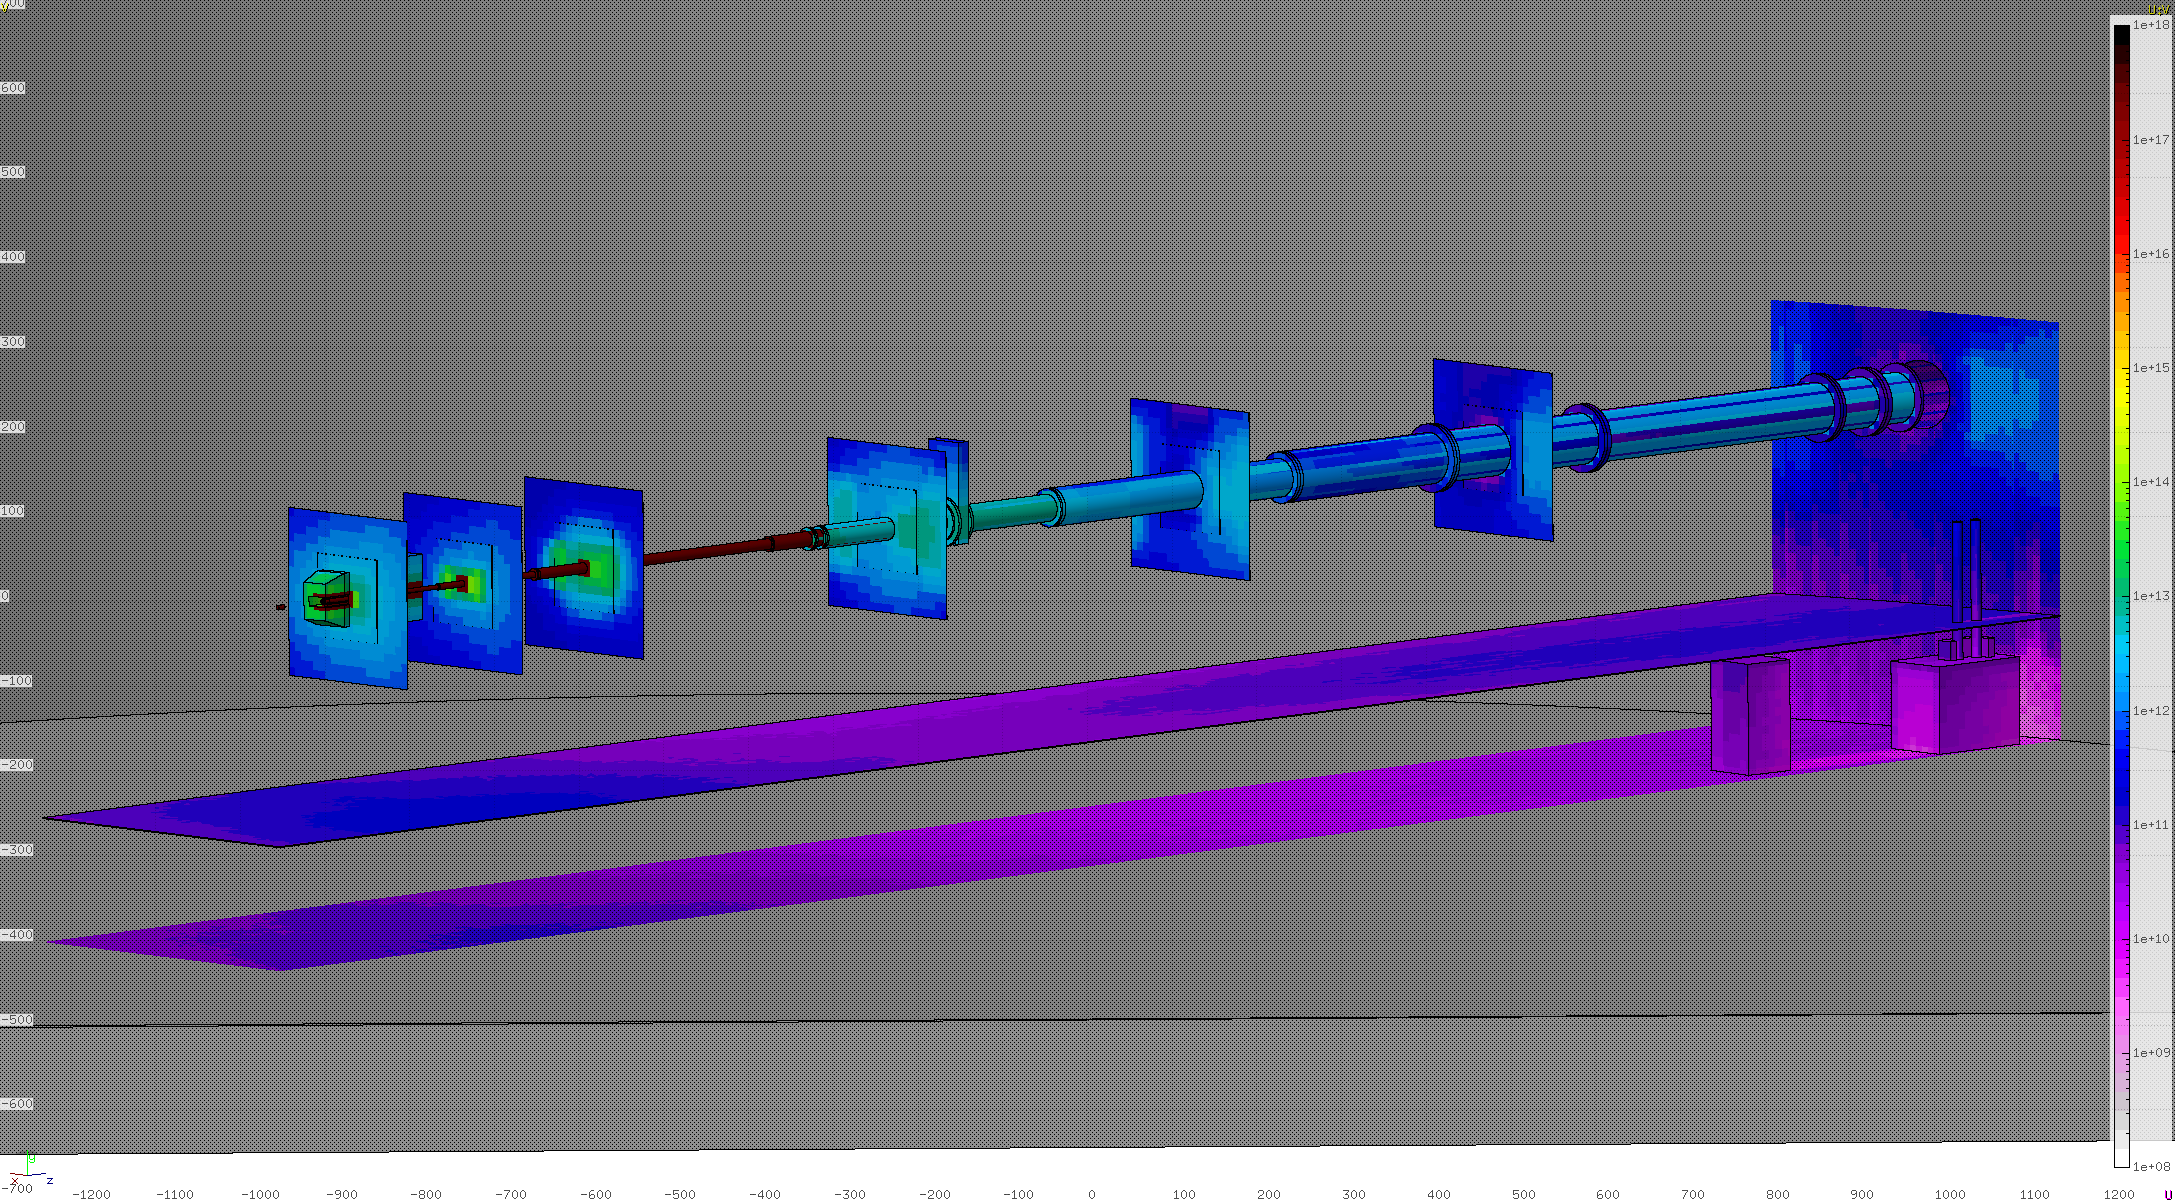
\includegraphics[width=\textwidth]{Pictures/accumulated_1MeVeq_neutron.png} \\
    \caption{Accumulated 1 MeV equivalent neutron fluence on Silicon cumulative for the full exposure as shown in Table\ref{tab:2}.   }
    \label{fig:1mev_acc}
  \end{center}
\end{figure}


\begin{figure}[!ht]
  \begin{center}
    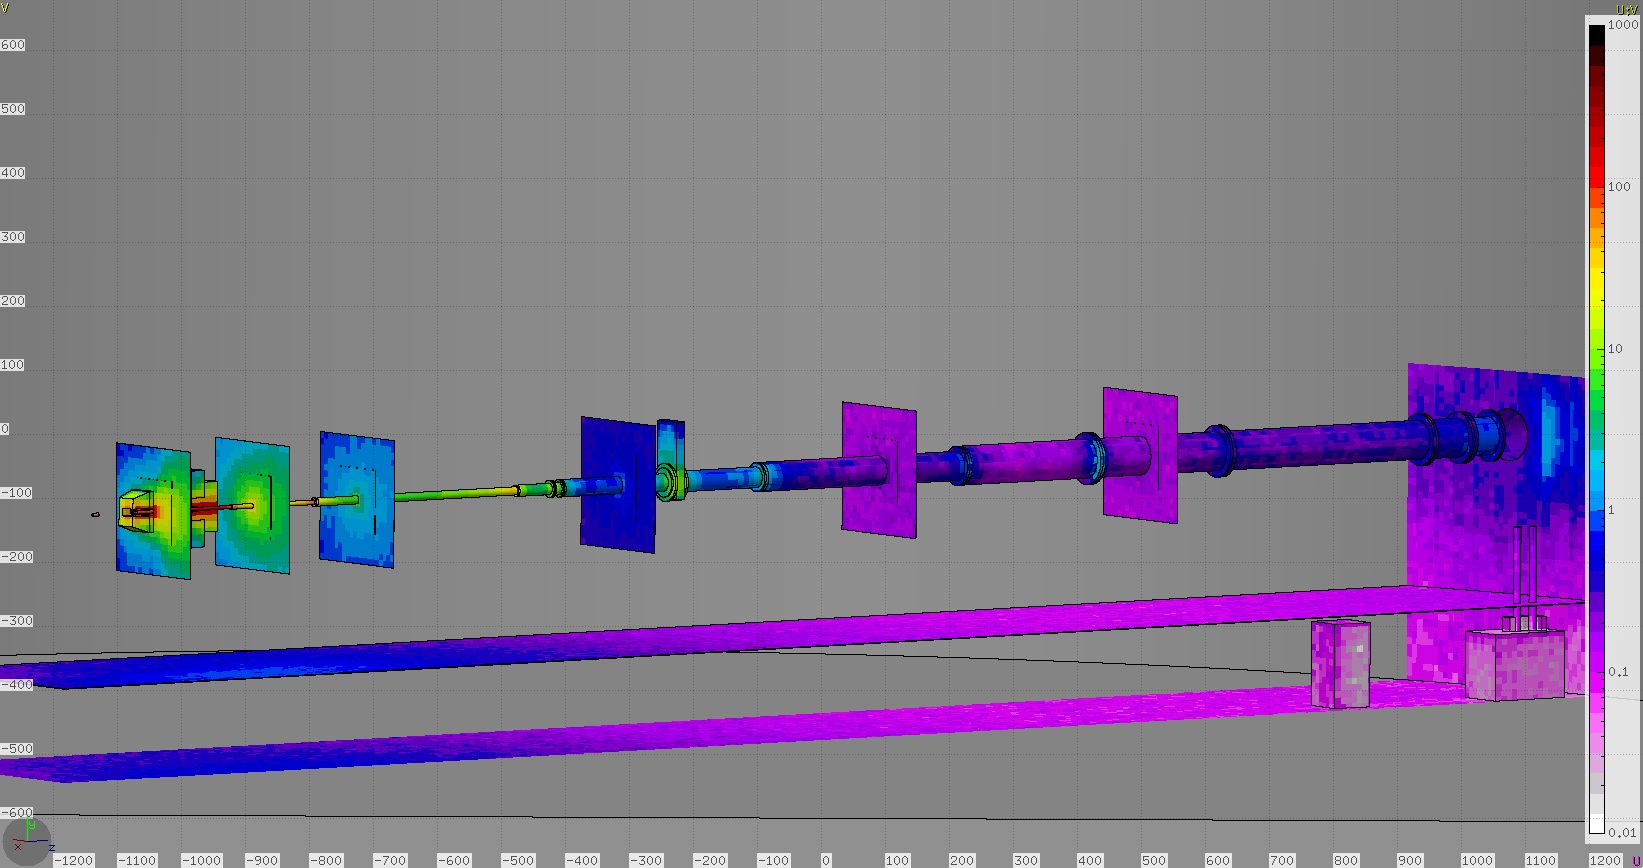
\includegraphics[width=\textwidth]{Pictures/accumulated_1h.png} \\
    \caption{Activation after 1 hour from full exposure as shown in Table\ref{tab:2}. Radiation level is expressed in mrem/hour.   }
    \label{fig:act1h}
  \end{center}
\end{figure}

\begin{figure}[!ht]
  \begin{center}
    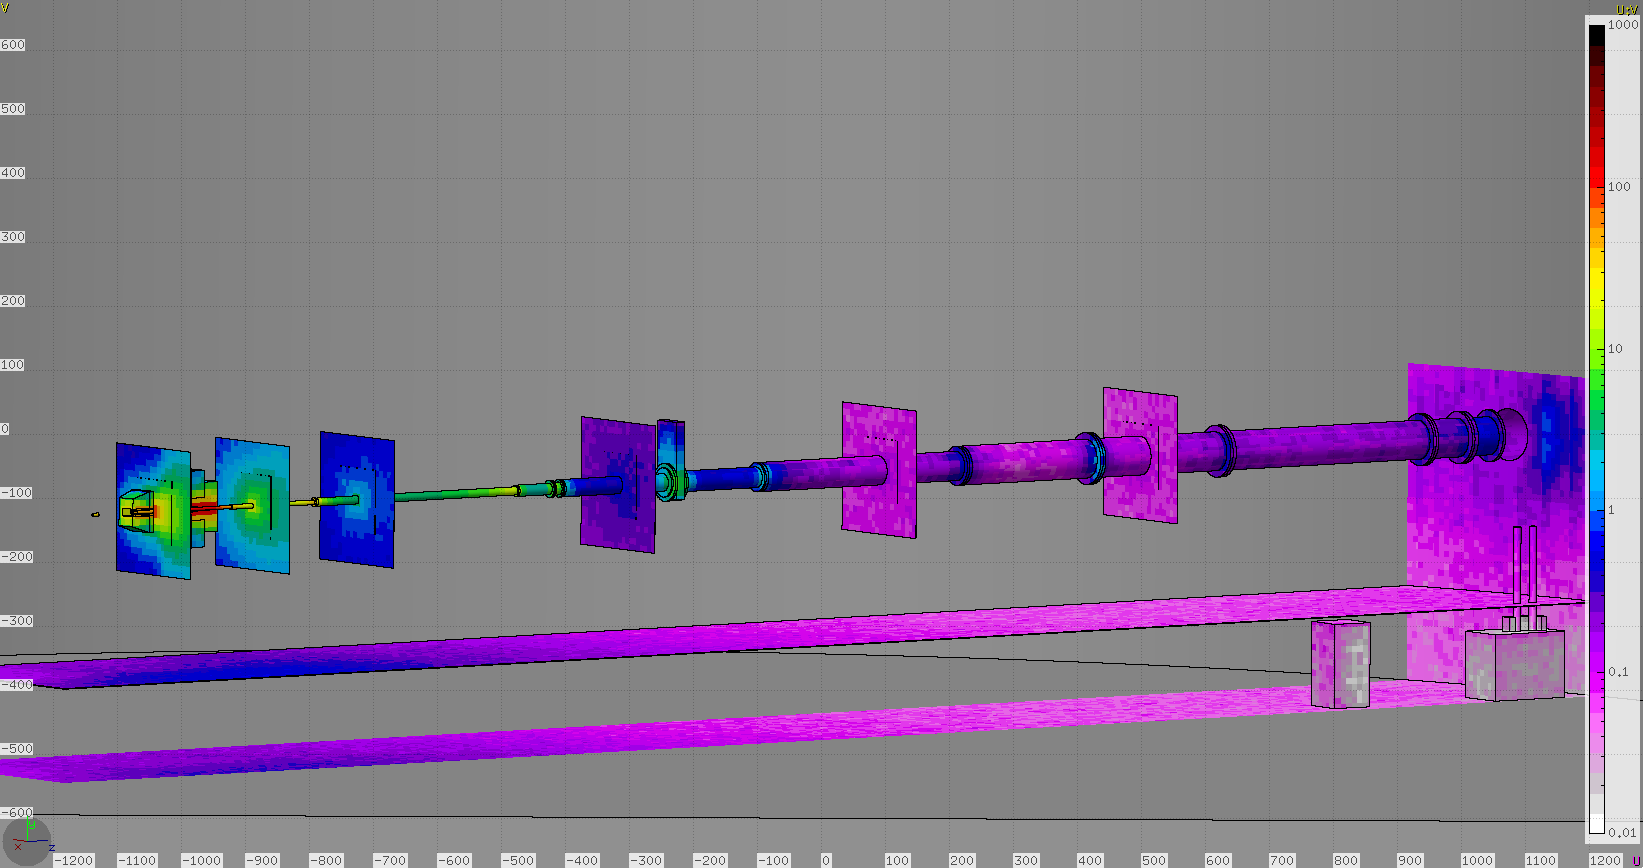
\includegraphics[width=\textwidth]{Pictures/accumulated_12h.png} \\
    \caption{Activation after 12 hours from  the full exposure as shown in Table\ref{tab:2}. Radiation level is expressed in mrem/hour.  }
    \label{fig:act12h}
  \end{center}
\end{figure}

\begin{figure}[!ht]
  \begin{center}
    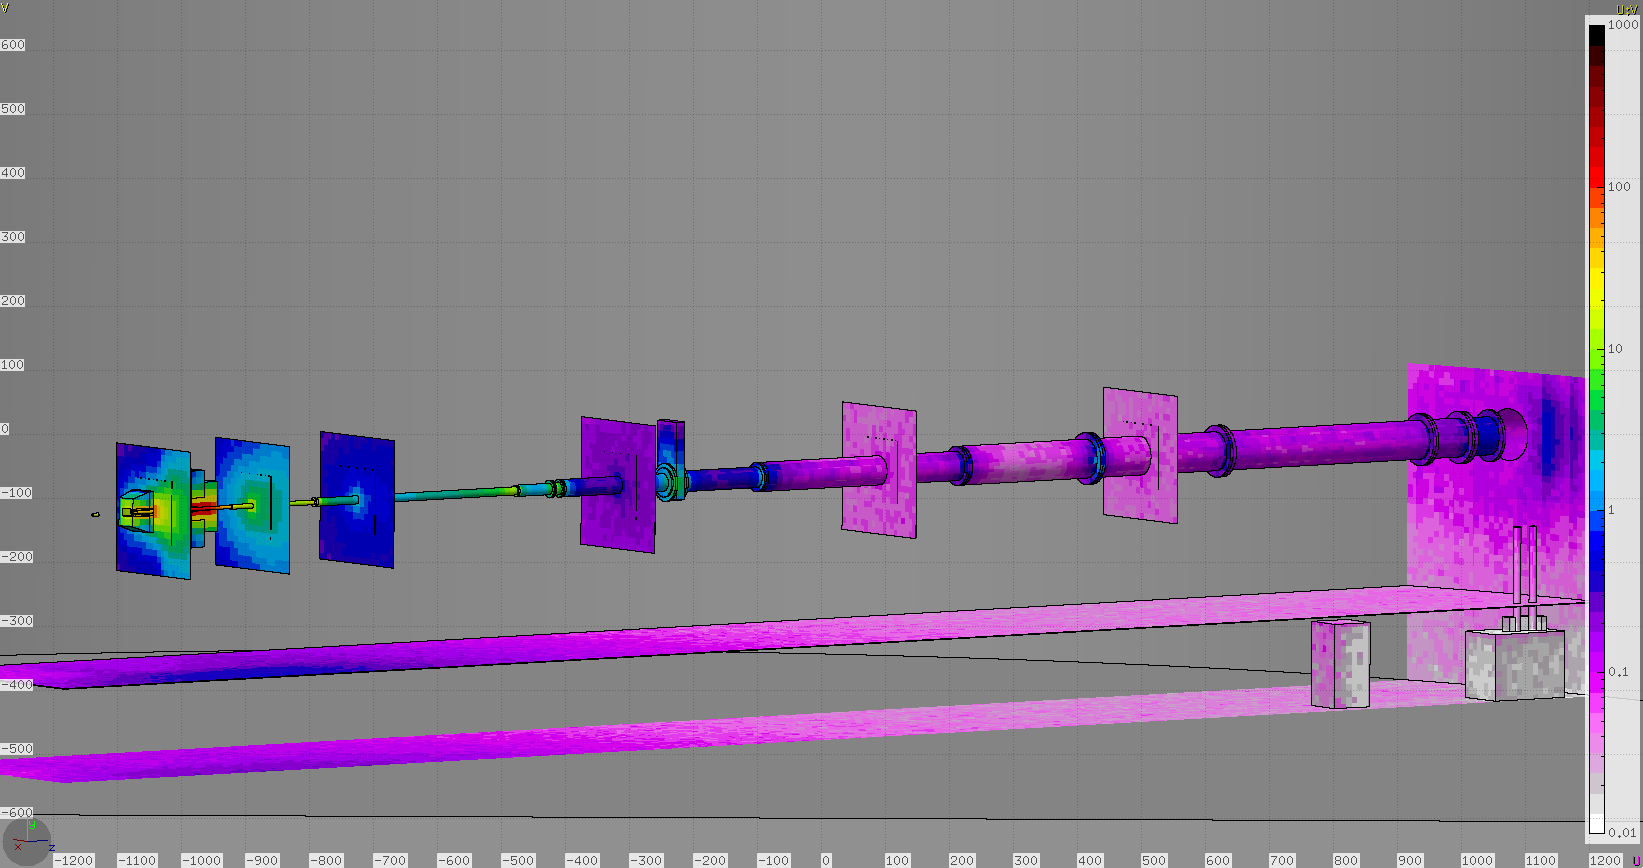
\includegraphics[width=\textwidth]{Pictures/accumulated_1d.png} \\
    \caption{Activation after 1 day from  the full exposure as shown in Table\ref{tab:2}.  Radiation level is expressed in mrem/hour. }
    \label{fig:act1d}
  \end{center}
\end{figure}

\begin{figure}[!ht]
  \begin{center}
    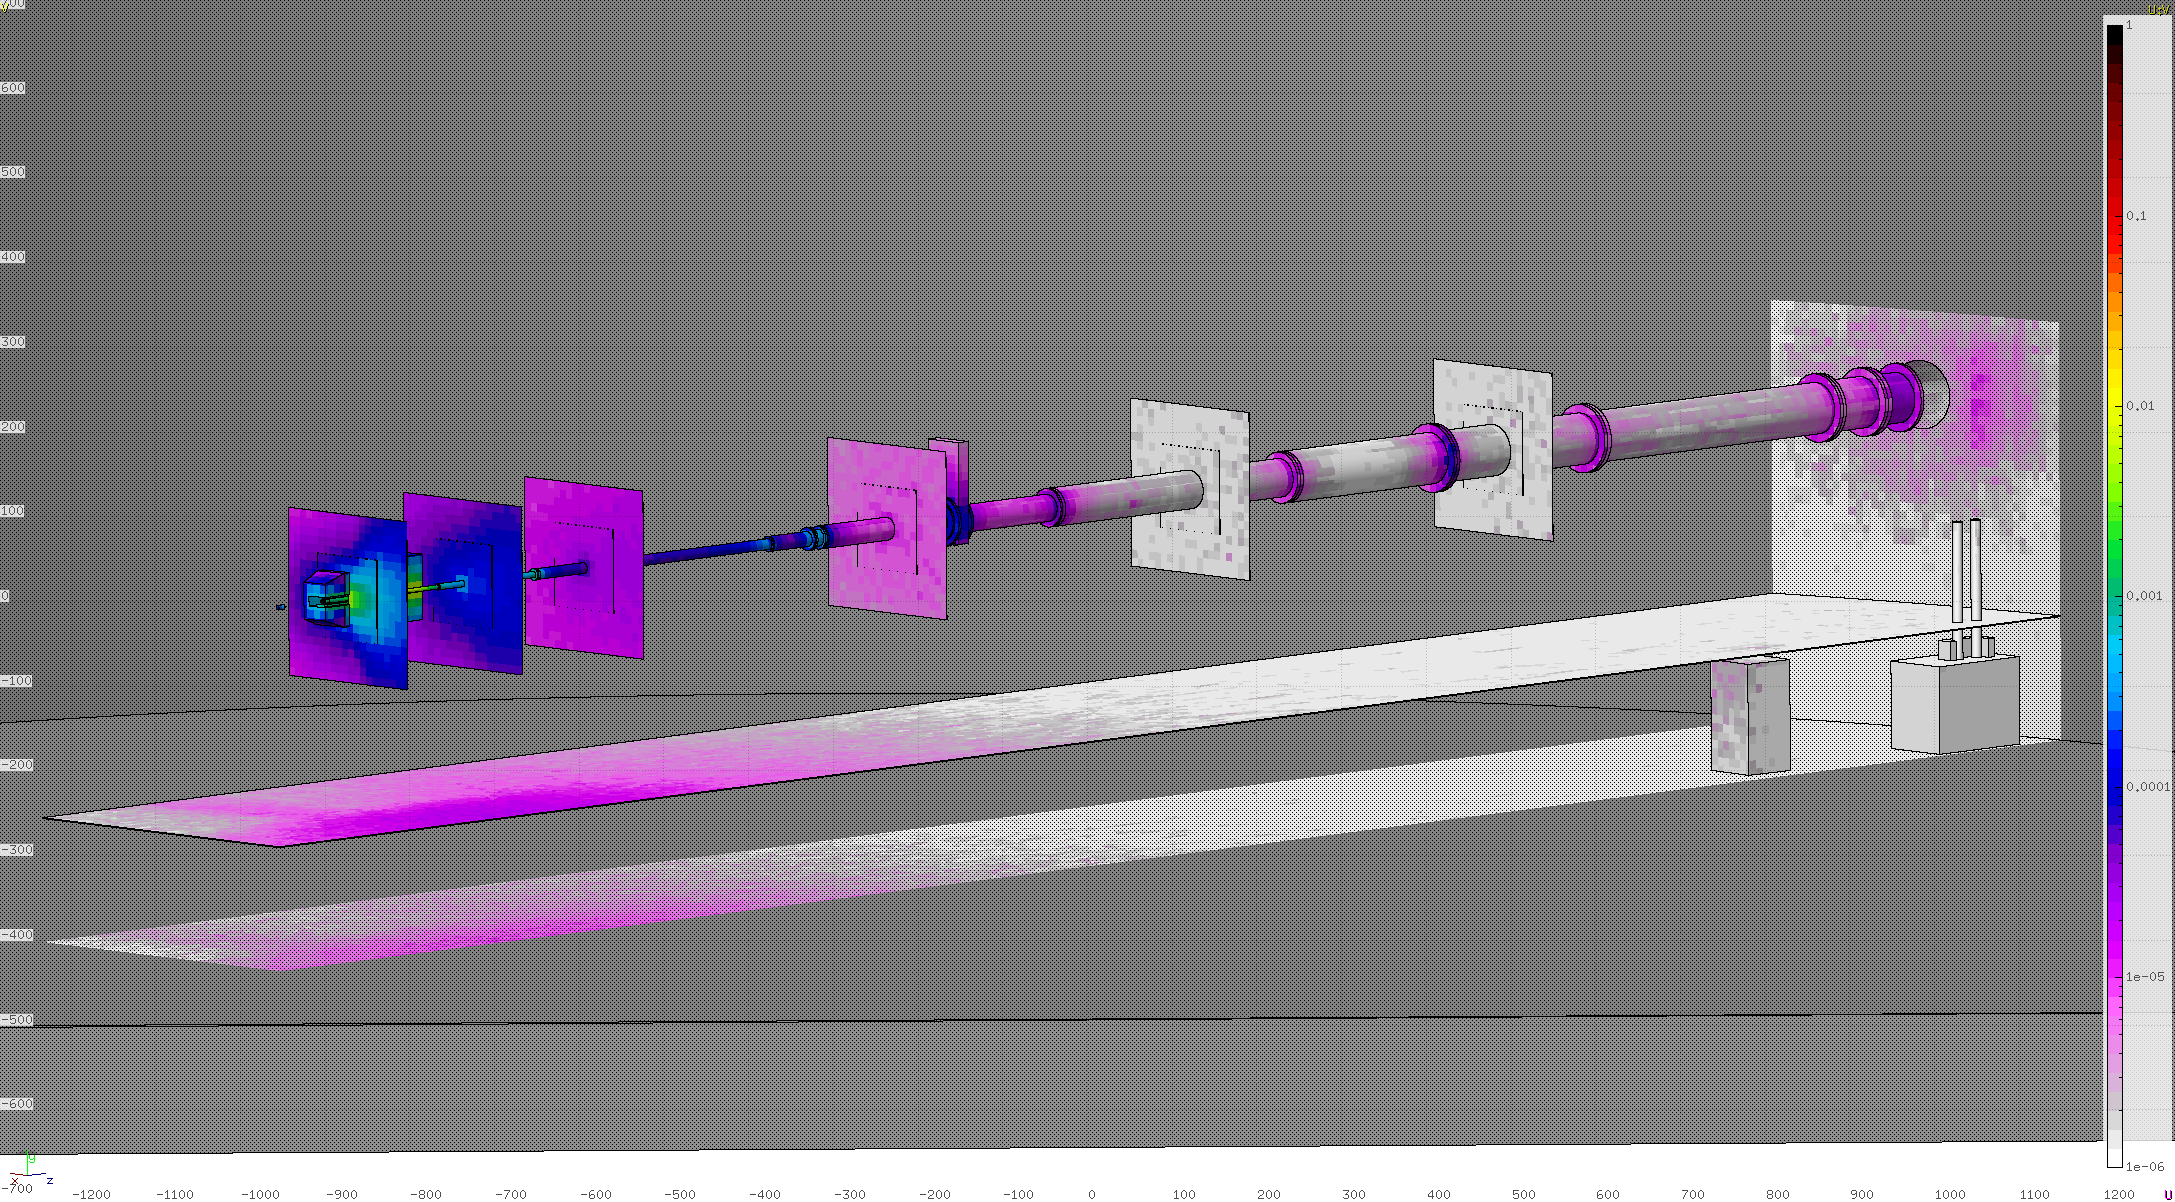
\includegraphics[width=\textwidth]{Pictures/accumulated_1w.png} \\
    \caption{Activation after 1 week from  the full exposure as shown in Table\ref{tab:2}. Radiation level is expressed in mrem/hour.  }
    \label{fig:act1w}
  \end{center}
\end{figure}

\begin{figure}[!ht]
  \begin{center}
    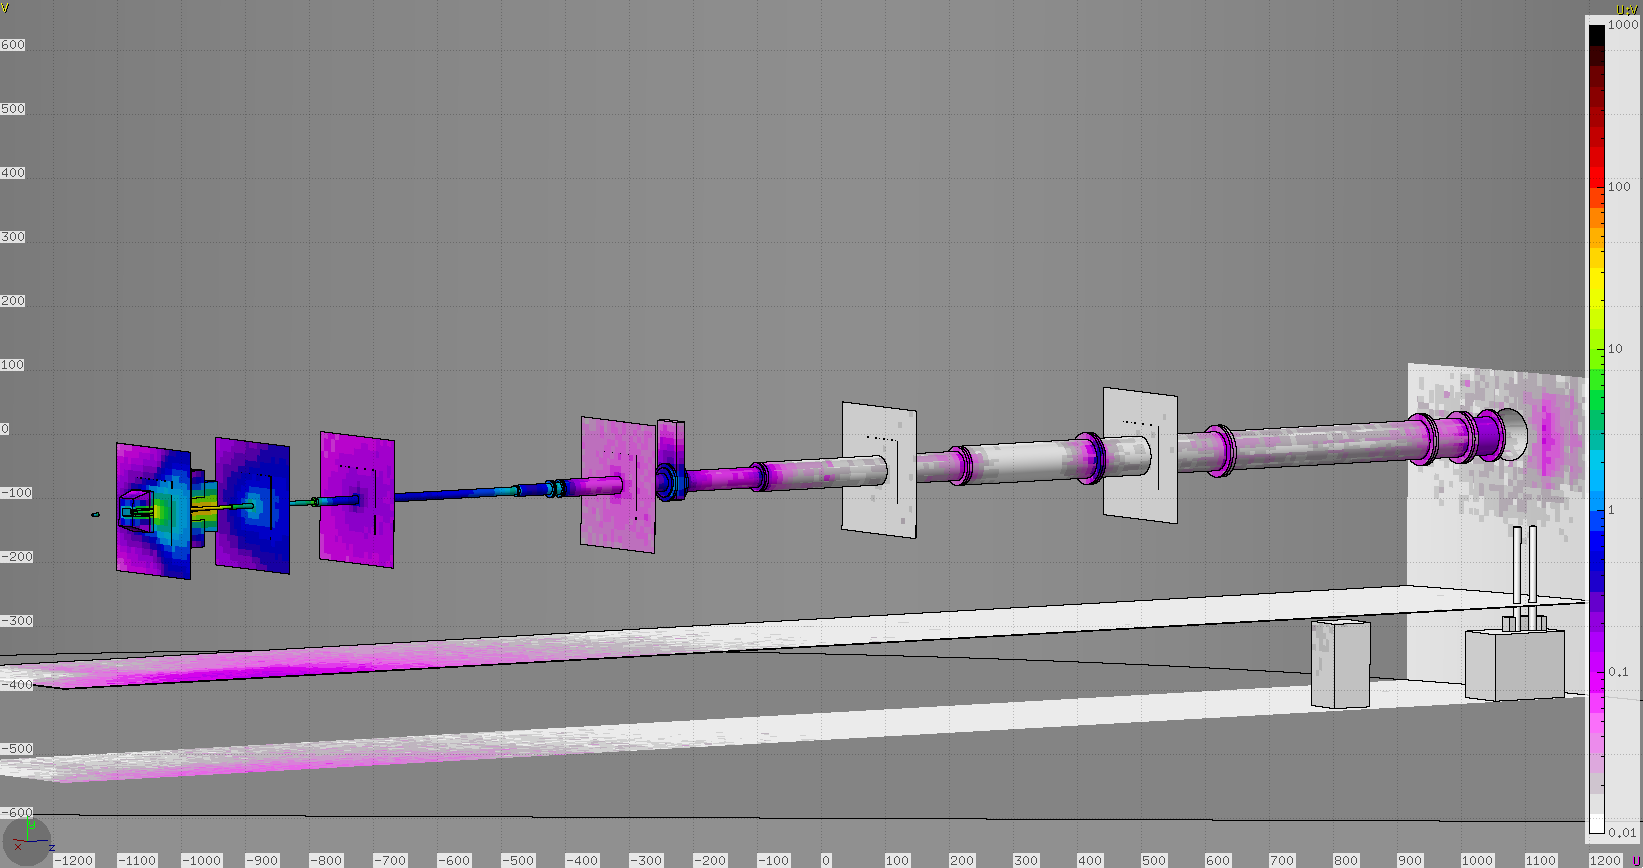
\includegraphics[width=\textwidth]{Pictures/accumulated_1m.png} \\
    \caption{Activation after 1 month from  the full exposure as shown in Table\ref{tab:2}. Radiation level is expressed in mrem/hour.  }
    \label{fig:act1m}
  \end{center}
\end{figure}

\begin{thebibliography}{9}
\bibitem[Code]{code} \emph{Fluka Hall-C Beam Accounting code:} \href{https://github.com/lorenzozana/Fluka-Hall-C-Beamline}{https://github.com/lorenzozana/Fluka-Hall-C-Beamline},
Lorenzo Zana
\bibitem[Fluka1]{fluka1} \emph{The FLUKA Code: Developments and Challenges for High Energy and Medical Applications:}
T.T. B�hlen, F. Cerutti, M.P.W. Chin, A. Fass�, A. Ferrari, P.G. Ortega, A. Mairani, P.R. Sala, G. Smirnov and V. Vlachoudis,
\textbf{Nuclear Data Sheets 120, 211-214 (2014)} 
\bibitem[Fluka2]{fluka2} \emph{FLUKA: a multi-particle transport code:}
A. Ferrari, P.R. Sala, A. Fasso`, and J. Ranft,
\textbf{CERN-2005-10 (2005), INFN/TC\_05/11, SLAC-R-773}
\end{thebibliography}

\end{document}
